\chapter{Implementation and Progress to Date}
Note that this chapter is still a work in progress. The exact description will be provided in the final report once everything has been finalized. The summary paragraphs below are provided as a draft.

This chapter presents the implementation details of the RAG system developed for the Meadow9+ transcription platform. It is organized into sections covering external resources and libraries, the retriever system implementation, and stretch goals and deployment.

\section{External Resources Incorporated}
The RAG system integrates multiple external libraries and services to provide comprehensive RAG capabilities, as summarized in Table \ref{tab:third-party-libraries}. These resources are organized into six primary categories, each serving distinct functional requirements within the pipeline.

\subsection{Core Framework Libraries}
The system is built on the LangChain ecosystem, which provides core abstractions for document handling, prompt template management, and output parsing. The web API layer utilizes FastAPI as the REST framework with Pydantic for data validation and serialization, enabling type-safe request/response handling through structured schemas defined in the data model definitions.\cite{langchain_document,langchain_prompts,langchain_output_parsers,fastapi_docs,pydantic_docs}

\subsection{Models Integration}
In the main RAG pipeline, a self-hosted jina-embeddings-v3-f16 model is used for document embedding, bge-reranker-v2-m3-FP16 is used for reranking retrieved candidates, and Qwen3-14B-Q4 serves as the answer generation LLM. For evaluation pipelines, DeepSeek, via the DeepSeek API, is used to generate ground-truth answers. All local models are hosted using llama.cpp server (llama-server), which provides efficient inference with optimized CPU/GPU acceleration and OpenAI-compatible API endpoints.\cite{jina_embeddings_v3,bge_reranker_v2_m3,qwen3_14b_base,deepseek_api_docs,llama_cpp_server}

\subsection{Other Libraries}
Other supporting libraries are consolidated in Table \ref{tab:third-party-libraries}, which groups tools by their primary roles in retrieval, model integration, data processing, and development workflows.\cite{langchain_openai_embeddings,langchain_chroma,chroma_persistence_sqlite,rank_bm25,metaphone_pypi,rapidfuzz_docs,wordfreq_pypi,dateparser_docs,pandas_docs,numpy_docs,matplotlib_docs,pytest_docs,requests_docs}

\begin{table}[H]
  \centering
  \begin{tabular}{|l|>{\raggedright\arraybackslash}p{0.32\textwidth}|>{\raggedright\arraybackslash}p{0.45\textwidth}|}
    \hline
    \textbf{Category} & \textbf{Key Libraries} & \textbf{Primary Purpose} \\
    \hline
    Framework & LangChain, FastAPI, Pydantic & RAG orchestration and REST API \\
    \hline
    Vector Store & Chroma & Persistent embedding storage and similarity search \\
    \hline
    Retrieval & rank-bm25, metaphone, rapidfuzz, wordfreq & Hybrid search with phonetic and fuzzy matching \\
    \hline
    LLM Integration & langchain-openai & OpenAI-compatible API wrapper for local/cloud models \\
    \hline
    Data Processing & dateparser, pandas, numpy, matplotlib & Natural language parsing and data analysis \\
    \hline
    Development & pytest, requests & Testing and external service communication \\
    \hline
  \end{tabular}
  \caption{Third-party libraries and frameworks categorized by functionality including LangChain, ChromaDB, and retrieval tools}
  \label{tab:third-party-libraries}
\end{table}

\section{Retriever System Implementation}
\subsection{Transcript Chunking Implementation}
\textbf{4.2.1.1 SRT Parsing}

The SRT parser implementation converts SRT format subtitle files into structured Python dictionaries. Figure \ref{fig:fig18} shows the input SRT format, which consists of sequence numbers, timestamps, and text content:

\begin{figure}[H]
  \centering
  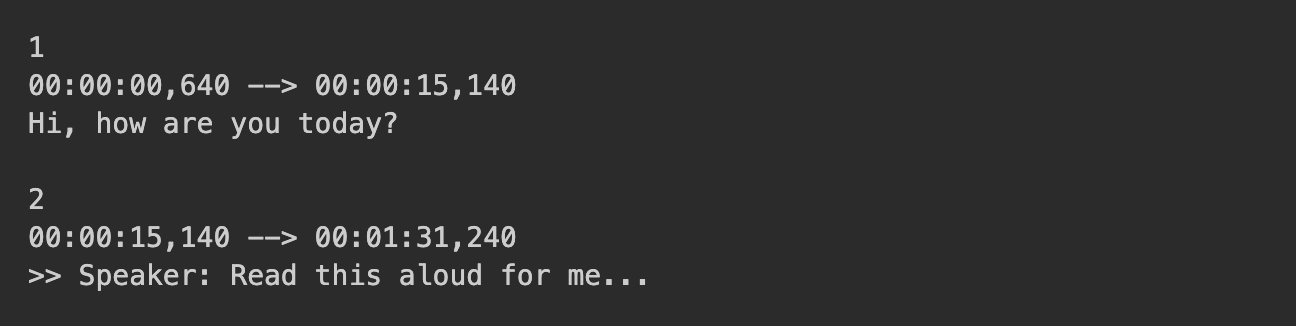
\includegraphics[width=1.0\textwidth]{figures/image18.png}
  \caption{SRT input format with sequence numbers and timestamps}
  \label{fig:fig18}
\end{figure}

The parser produces structured output, as shown in Figure \ref{fig:fig19}:

\begin{figure}[H]
  \centering
  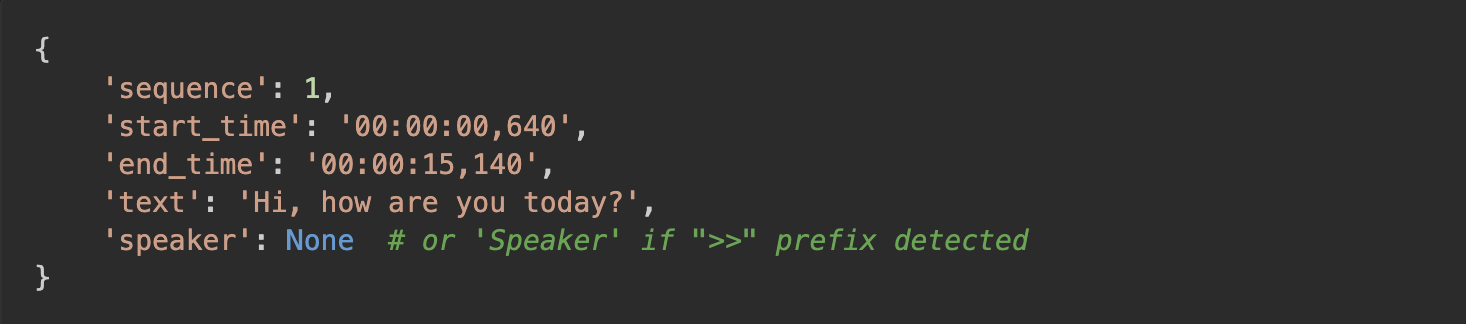
\includegraphics[width=1.0\textwidth]{figures/image19.png}
  \caption{Parsed SRT structure with speaker metadata extraction}
  \label{fig:fig19}
\end{figure}

Speaker detection handles two patterns: simple >> prefix and >> SpeakerName: format. The speaker name is extracted and removed from the text content, preserving speaker metadata separately.

\textbf{4.2.1.2 Token-Based Merging}

\textbf{Token-Based Chunking Strategy}

The chunking strategy employs actual tokenizer-based token counting rather than character-based estimation. This approach ensures accurate management of the LLM context window under strict input constraints, while maintaining consistency with the embedding model’s token limits. By enforcing explicit token-based boundaries during chunk construction and retrieval, it prevents both underutilization of available chunk capacity and overflow beyond model limits. As a result, the system retains precise and predictable control over the total amount of retrieved context supplied to downstream generation components.

\textbf{Preservation of Natural SRT Boundaries}

Rather than applying arbitrary text splitting, the system preserves the original SRT subtitle boundaries during chunking to retain transcript structure and metadata fidelity. This design maintains speaker diarization integrity across chunks and preserves the natural conversational flow and turn-taking structure, which improves coherence during downstream retrieval and generation. In addition, it ensures timestamp metadata remains accurately aligned with the source transcript, enabling reliable temporal referencing during evaluation and user-facing responses. By respecting these semantic units, the subsequent merging strategy can combine segments more meaningfully without disrupting the underlying conversational context.

Small SRT chunks are merged to create appropriately sized segments for embedding and retrieval. Figure \ref{fig:fig20} shows how the merging algorithm operates:

\begin{figure}[H]
  \centering
  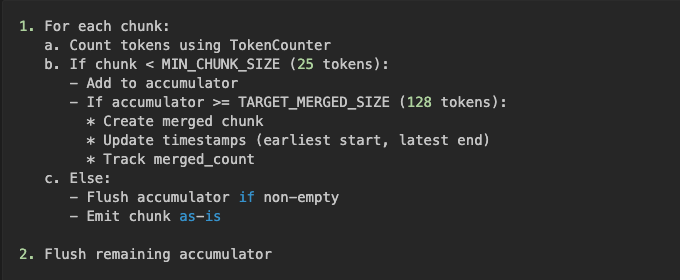
\includegraphics[width=1.0\textwidth]{figures/image20.png}
  \caption{Token-based merging algorithm for chunk size optimization}
  \label{fig:fig20}
\end{figure}

\textbf{4.2.1.3 Document Creation and Metadata Schema}

The final stage converts parsed chunks into LangChain Document objects, as shown in Figure \ref{fig:fig22}:\cite{langchain_document}

\begin{figure}[H]
  \centering
  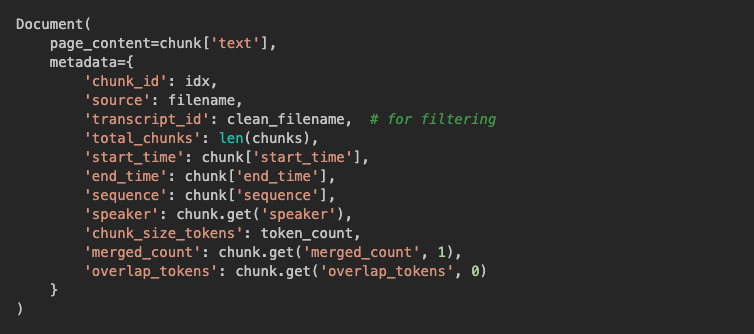
\includegraphics[width=1.0\textwidth]{figures/image22.png}
  \caption{LangChain Document object creation with chunk metadata}
  \label{fig:fig22}
\end{figure}

Table \ref{tab:document-metadata-schema} shows the document metadata schema field descriptions:

\begin{table}[H]
  \centering
  \begin{tabular}{|l|l|l|}
    \hline
    \textbf{Field} & \textbf{Type} & \textbf{Description} \\
    \hline
    chunk\_id & int & Sequential ID within transcript (0-indexed) \\
    \hline
    source & str & Original filename (e.g., "example\_transcript\_1.srt") \\
    \hline
    transcript\_id & str & Cleaned filename for metadata filtering \\
    \hline
    total\_chunks & int & Total number of chunks in source transcript \\
    \hline
    start\_time & str & Start timestamp in HH:MM:SS,mmm format \\
    \hline
    end\_time & str & End timestamp in HH:MM:SS,mmm format \\
    \hline
    sequence & int & Original SRT sequence number \\
    \hline
    speaker & str/None & Detected speaker name from SRT markers \\
    \hline
    chunk\_size\_tokens & int & Token count via TokenCounter \\
    \hline
    merged\_count & int & Number of original chunks merged ($\geq 1$) \\
    \hline
    overlap\_tokens & int & Tokens overlapping with previous chunk \\
    \hline
  \end{tabular}
  \caption{Document metadata schema field descriptions}
  \label{tab:document-metadata-schema}
\end{table}

\subsection{Embedding Generation and Vector Storage}

\textbf{4.2.2.1 Global Unified Index Architecture}

All transcript chunks are stored in a single, global vector store rather than maintaining separate indices per transcript. This architectural decision provides several key advantages: simplified index management (one collection instead of dozens), reduced memory overhead (shared vocabulary and model weights), support for cross-transcript semantic search when queries span multiple documents, and unified metadata-based filtering for transcript scoping. Metadata-based filtering enables efficient restriction of search results to specific transcripts without requiring separate indices, as demonstrated in Figure \ref{fig:fig27b} (shown in Section 4.2.3.1).

\textbf{4.2.2.2 Embedding Service}

The embedding functionality is implemented as a separate microservice, hosted via llama.cpp server. This separation from the main LLM service and reranker service enables independent scaling, resource allocation, and model versioning for each component.

The embedding service communicates via HTTP POST requests to the /v1/embeddings endpoint, following the OpenAI embeddings API specification. LangChain's OpenAIEmbeddings wrapper abstracts this HTTP communication, providing methods like embed\_query() (for single-query embedding) and embed\_documents() (for batch document embedding).\cite{openai_embeddings_api,langchain_openai_embeddings} The llama.cpp server handles request batching internally, optimizing GPU utilization by processing multiple embeddings concurrently when batch sizes exceed single-request thresholds.

\textbf{4.2.2.3 Transcript Processing}

Figure \ref{fig:fig24f} shows the document processing pipeline for a single transcript. The pipeline consists of three stages: (1) parsing the SRT file into structured chunks using the SRT parser (described in Section 4.2.1), (2) creating LangChain Document objects with metadata via the document processor, and (3) adding a transcript\_id field to each document's metadata for efficient filtering during retrieval. For simplicity, the transcript\_id is derived from the filename by removing the .srt extension and replacing periods with underscores, producing clean identifiers like "example\_transcript\_1" that can be used in Chroma metadata filters.

\begin{figure}[H]
  \centering
  
\includegraphics[width=1.0\textwidth]{figure24f.png}
  \caption{Document processing pipeline}
  \label{fig:fig24f}
\end{figure}

This processing stage integrates with the chunking logic described in Section 4.2.1, where SRT entries are merged based on token counts to produce chunks of appropriate size for embedding. The resulting Document objects contain both page\_content (the merged chunk text) and metadata (chunk\_id, source filename, timestamps, speaker information, and transcript\_id), enabling both semantic retrieval and metadata-based filtering.

\textbf{4.2.2.4 Batch Embedding Generation and Vector Store Creation}

Embedding generation is the most computationally expensive component of the index building pipeline, requiring forward passes through the transformer-based embedding model for every document chunk. To maximize throughput and GPU utilization, embeddings are generated in batches rather than one-by-one. Figure \ref{fig:fig25d} shows the vector store creation logic using Chroma's from\_documents() method, which automatically batches embedding requests and stores the resulting vectors in the SQLite-backed database.\cite{langchain_chroma,chroma_persistence_sqlite}

\begin{figure}[H]
  \centering
  
\includegraphics[width=1.0\textwidth]{figure25d.png}
  \caption{Vector store creation from documents}
  \label{fig:fig25d}
\end{figure}

Figure \ref{fig:fig25e} demonstrates incremental document addition to an existing vector store. The add\_documents() method extends the existing collection with new embeddings without requiring a full rebuild, preserving the existing embeddings and metadata while appending the new vectors. The optional ids parameter enables upsert behavior (insert if new, update if exists) when document IDs are provided, though the deduplication logic described earlier typically ensures that only new documents reach this stage.

\begin{figure}[H]
  \centering
  
\includegraphics[width=1.0\textwidth]{figure25e.png}
  \caption{Incremental document addition}
  \label{fig:fig25e}
\end{figure}

LangChain's automatic batching mechanism abstracts the complexity of batch size tuning, request pipelining, and error handling, enabling the index builder to focus on higher-level logic (deduplication, metadata management) rather than low-level HTTP optimization. However, this abstraction does limit control over batch sizes and parallelism; for production deployments with strict latency or throughput requirements, a custom batching implementation with explicit concurrency control may provide better performance.

\textbf{4.2.2.5 ChromaDB Storage and Persistence}

Chroma stores all embeddings, metadata, and collection configuration in a single SQLite database file (chroma.sqlite3) located in the persist directory.\cite{chroma_persistence_sqlite} Figure \ref{fig:fig26a} illustrates the directory structure, showing how the vector store, BM25 index, and phonetic index are co-located within the same storage hierarchy. This unified structure simplifies backup, replication, and deployment: copying the vector\_stores/global\_combined/ directory to another machine produces a fully functional index without requiring configuration changes or re-embedding.

\begin{figure}[H]
  \centering
  
\includegraphics[width=1.0\textwidth]{figure26a.png}
  \caption{ChromaDB storage directory structure}
  \label{fig:fig26a}
\end{figure}

The embedding generation and vector storage subsystem implements the foundation for the hybrid retrieval pipeline described in Section 4.2.3, providing the semantic signal that complements keyword-based, phonetic, and fuzzy matching. By embedding both queries and documents in the same semantic space, the retriever enables the system to retrieve relevant chunks even when query terms do not appear verbatim in the document text, capturing paraphrasing, synonym variation, and conceptual similarity that lexical methods cannot detect.

\subsection{Multi-Stage Retrieval Process}
The retrieval pipeline implements a four-stage progressive refinement strategy, each stage narrowing the candidate set with increasing computational cost and precision.

\textbf{4.2.3.1 Stage 1: Hybrid Search}

\textbf{Vector Search (Semantic)}

Vector search implements semantic retrieval using dense embedding representations generated by the Jina embedding model. Each document chunk is encoded as a high-dimensional vector (1024 dimensions for jina-embeddings-v3), and retrieval is performed by computing cosine similarity between the query embedding and all document embeddings in the vector store.\cite{jina_embeddings_v3} This approach captures semantic relationships beyond exact keyword matches, enabling the system to retrieve relevant chunks even when queries are paraphrased, use synonyms, or express concepts differently from the source text.

The core vector search function, shown in Figure \ref{fig:fig27a}, provides a unified interface for semantic retrieval with optional metadata filtering. When a Chroma filter is provided, it restricts the search space to specific transcripts by matching metadata fields, enabling transcript-scoped search. Without filters, the system performs global search across all indexed documents.

\begin{figure}[H]
  \centering
  
\includegraphics[width=1.0\textwidth]{figure27a.png}
  \caption{Vector search core function showing semantic retrieval with optional Chroma metadata filtering}
  \label{fig:fig27a}
\end{figure}

Figure \ref{fig:fig27b} demonstrates how transcript filters are constructed for the Chroma vector database. The system supports both single-transcript filtering using the \$eq operator and multi-transcript filtering using the \$in operator. This metadata-based filtering ensures efficient scoping of search results without requiring separate vector indices per transcript.

\begin{figure}[H]
  \centering
  
\includegraphics[width=1.0\textwidth]{figure27b.png}
  \caption{Chroma metadata filter construction for transcript scoping}
  \label{fig:fig27b}
\end{figure}

Key advantages of vector search include robust handling of paraphrasing, synonym variation, and semantic similarity beyond surface-level keyword matching. It effectively captures conceptual relationships and topical relevance, making it particularly strong for queries that express intent in different words than the source transcript. However, vector search can struggle with proper nouns, rare technical terms, and exact keyword requirements, which motivates the complementary use of BM25 keyword search.

\textbf{BM25 Search (Keyword)}

BM25 implements probabilistic keyword-based retrieval using the BM25Okapi ranking function, a well-established algorithm in information retrieval that scores documents based on term frequency (TF) and inverse document frequency (IDF).\cite{robertson2009bm25,rank_bm25} Unlike semantic search, which relies on dense vector representations, BM25 performs exact lexical matching, making it particularly effective for queries containing proper nouns, technical terminology, product names, and specific keywords that must appear verbatim in retrieved chunks.

The BM25 retrieval pipeline consists of five main stages: tokenization, index initialization, query processing, scoring and ranking, and persistence. Each stage is implemented as a modular component within the BM25Retriever class.

\textbf{Tokenization Strategy}

Figure \ref{fig:fig28a} shows the default tokenizer implementation, which applies a simple lowercase split on whitespace. This lightweight approach avoids dependencies on NLP libraries while providing adequate performance for most queries.

\begin{figure}[H]
  \centering
  
\includegraphics[width=1.0\textwidth]{figure28a.png}
  \caption{BM25 tokenization function using lowercase split}
  \label{fig:fig28a}
\end{figure}

\textbf{Index Initialization}

The BM25 index is constructed once and persisted alongside the vector store. It is constructed by tokenizing all document chunks in the corpus and building an inverted index structure, as shown in Figure \ref{fig:fig28b}. The initialization process iterates over all LangChain Document objects, applies the tokenizer to each document's page content, and passes the tokenized corpus to the BM25Okapi constructor. The BM25Okapi class internally builds an inverted index mapping terms to document IDs and computes IDF weights for each unique term in the corpus.\cite{rank_bm25} This preprocessing step is performed once during index building and enables fast scoring at query time.

\begin{figure}[H]
  \centering
  
\includegraphics[width=1.0\textwidth]{figure28b.png}
  \caption{BM25 index initialization with corpus tokenization}
  \label{fig:fig28b}
\end{figure}

\textbf{Query Processing and Metadata Filtering}

At query time, the BM25 retriever tokenizes the input query using the same tokenization logic applied during indexing to ensure consistency. The retrieval function supports optional metadata-based filtering to restrict results to specific transcripts, as demonstrated in Figure \ref{fig:fig28c}. When a filter is provided, the system first identifies document indices matching the specified metadata field and value (e.g., transcript\_id), then invokes the optimized get\_batch\_scores method to compute BM25 scores only for the filtered subset of documents. This selective scoring strategy significantly reduces computational cost when searching within a single transcript or small transcript subset, avoiding unnecessary score computation for out-of-scope documents.

\begin{figure}[H]
  \centering
  
\includegraphics[width=1.0\textwidth]{figure28c.png}
  \caption{BM25 query tokenization and metadata filtering}
  \label{fig:fig28c}
\end{figure}

\textbf{Scoring and Ranking}

After computing BM25 scores for candidate documents, the retriever ranks results by score in descending order and selects the top-k highest-scoring chunks, as shown in Figure \ref{fig:fig28d}. When metadata filtering is applied, the system sorts the filtered scores and returns the top-k results. Without filtering, it uses NumPy's argsort operation to efficiently identify the top-k document indices from the full score array. The BM25Okapi scoring function applies the standard BM25 formula with parameters k1=1.5 (controlling term frequency saturation) and b=0.75 (controlling document length normalization).\cite{robertson2009bm25,rank_bm25} These parameter values are widely used defaults in the information retrieval literature and provide a reasonable balance between precision and recall across diverse query types.

\begin{figure}[H]
  \centering
  
\includegraphics[width=1.0\textwidth]{figure28d.png}
  \caption{BM25 scoring and top-k ranking}
  \label{fig:fig28d}
\end{figure}

Once the top-k document indices and scores are determined, the retriever constructs LangChain Document objects by copying the original document content and metadata, then appending the BM25 score as an additional metadata field, as illustrated in Figure \ref{fig:fig28e}. This metadata preservation ensures that downstream components (e.g., RRF fusion, rerankers) can access both the original chunk metadata (timestamps, speakers, transcript IDs) and the BM25 relevance score.

\begin{figure}[H]
  \centering
  
\includegraphics[width=1.0\textwidth]{figure28e.png}
  \caption{BM25 result document construction}
  \label{fig:fig28e}
\end{figure}

\textbf{Index Persistence}

To avoid rebuilding the BM25 index on every system restart, the retriever implements pickle-based serialization for persistent storage, as shown in Figure \ref{fig:fig28f}. The save\_index method serializes the entire retriever state, including the document list, BM25 index structure, and tokenizer function, to disk. On subsequent system startups, the load\_index classmethod deserializes the saved state, enabling fast index loading without re-tokenizing the corpus or recomputing IDF weights. This persistence mechanism significantly reduces startup time for large document collections.

\begin{figure}[H]
  \centering
  
\includegraphics[width=1.0\textwidth]{figure28f.png}
  \caption{BM25 index persistence via pickle serialization}
  \label{fig:fig28f}
\end{figure}

Key advantages of BM25 search include strong performance on exact keyword queries, robust handling of proper nouns and technical terminology, and computational efficiency relative to neural retrieval models. BM25 excels when query terms must appear verbatim in the retrieved context, making it complementary to vector search, which prioritizes semantic similarity over exact lexical matches.

\textbf{Phonetic Search (ASR Error Handling)}

Phonetic search addresses a critical limitation of exact lexical matching in ASR-generated transcripts: proper nouns, technical terms, and rare vocabulary are frequently misrecognized by speech-to-text models, resulting in transcription errors that preserve phonetic similarity but differ in spelling. For example, a query for "Samsung" may fail to retrieve chunks where the ASR system transcribed the same spoken word as "Samson" or "Samsang." Since these variants share similar pronunciation, they should ideally be retrieved despite lexical differences. Phonetic search solves this problem by encoding words into phonetic representations using the Double Metaphone algorithm, enabling sound-alike matching that is robust to ASR transcription errors.\cite{black2021doublemetaphone,metaphone_pypi}

\textbf{Database Schema and Index Structure}

The phonetic indexer is implemented using a SQLite-backed database with a single primary table and three supporting indices, as shown in Figure \ref{fig:fig29a}. The phonetic\_codes table stores mappings from phonetic codes (e.g., "SMSNK" for "Samsung") to chunk IDs, transcript IDs, and original words. Each row represents one word in one chunk, encoded by its phonetic representation. The composite primary key on (phonetic\_code, chunk\_id, word) ensures that duplicate entries are automatically deduplicated during batch insertion. Three indices—idx\_phonetic\_code, idx\_transcript, and idx\_chunk\_id—enable fast lookup by phonetic code (the primary access pattern), filtering by transcript ID, and reverse lookup by chunk ID, respectively.

\begin{figure}[H]
  \centering
  
\includegraphics[width=1.0\textwidth]{figure29a.png}
  \caption{Phonetic index database schema with SQLite table and indices}
  \label{fig:fig29a}
\end{figure}

This schema design prioritizes retrieval efficiency: queries typically access the index by phonetic code (e.g., "find all chunks containing code 'SMSNK'"), which is accelerated by the idx\_phonetic\_code index. The transcript\_id field supports metadata filtering, allowing the system to restrict phonetic search to a specific transcript or transcript set without scanning unrelated chunks. The word field preserves the original token for debugging and analysis, though it is not used in the core retrieval logic.

\textbf{Tokenization and Word Filtering}

Before phonetic encoding, the indexer tokenizes input text by extracting alphabetic words and filtering short tokens, as illustrated in Figure \ref{fig:fig29b}. The tokenize\_and\_encode method applies a regular expression ([a-zA-Z]+) to extract contiguous alphabetic sequences, discarding punctuation, numbers, and whitespace. Words shorter than 3 characters are filtered out because short words (e.g., "is", "at", "on") are too common to provide discriminative phonetic matches and would introduce noise into the index. This length threshold balances index size (excluding uninformative short words) against recall (retaining meaningful terms).

\begin{figure}[H]
  \centering
  
\includegraphics[width=1.0\textwidth]{figure29b.png}
  \caption{Phonetic word tokenization and filtering}
  \label{fig:fig29b}
\end{figure}

\textbf{Double Metaphone Encoding}

Figure \ref{fig:fig29c} shows the core phonetic encoding logic, which applies the Double Metaphone algorithm to each filtered word. The doublemetaphone function (from the metaphone library) returns a tuple of two phonetic codes: a primary code and an optional alternate code.\cite{black2021doublemetaphone,metaphone_pypi} The implementation extracts only the primary code, as testing revealed that the alternate code provided minimal additional recall while significantly increasing index size. The phonetic pairs are deduplicated using a seen set to prevent redundant entries when the same word appears multiple times in a document.

\begin{figure}[H]
  \centering
  
\includegraphics[width=1.0\textwidth]{figure29c.png}
  \caption{Double Metaphone phonetic encoding}
  \label{fig:fig29c}
\end{figure}


The Double Metaphone algorithm is particularly well-suited for ASR error handling because it produces consistent codes for homophones and phonetically similar words.\cite{black2021doublemetaphone} For example, "Samsung", "Samson", and "Samsang" produce phonetically similar codes, enabling retrieval across spelling variations. Similarly, other brand names like "Apple" and "Aple" would also produce matching phonetic codes. Figure \ref{fig:fig31} provides additional examples of phonetic encodings.

\begin{figure}[H]
  \centering
  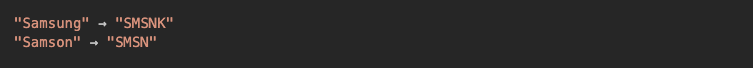
\includegraphics[width=1.0\textwidth]{figures/image31.png}
  \caption{Phonetic encoding examples for homophone matching}
  \label{fig:fig31}
\end{figure}

\textbf{Index Building and Batch Insertion}

The index\_documents method, shown in Figure \ref{fig:fig29d}, constructs the phonetic index by iterating over all document chunks, encoding their content, and batch-inserting the resulting phonetic codes into the SQLite database. The force\_rebuild parameter allows the index to be cleared and rebuilt from scratch, useful when the tokenization logic or encoding algorithm changes. In normal operation, the indexer performs incremental updates by inserting only new documents, relying on the "INSERT OR IGNORE" SQL command to skip duplicate entries that match the primary key.

\begin{figure}[H]
  \centering
  
\includegraphics[width=1.0\textwidth]{figure29d.png}
  \caption{Phonetic index building with batch insertion}
  \label{fig:fig29d}
\end{figure}

Batch insertion significantly improves indexing performance compared to row-by-row insertion, as it reduces the number of SQL transactions and database commits.

\textbf{Query Processing and Metadata Filtering}

At query time, the phonetic indexer encodes the query into phonetic codes using the same tokenize\_and\_encode method applied during indexing, then executes a SQL query to find all chunks containing any of the query codes. Figure \ref{fig:fig29e} shows the SQL query construction logic for the filtered case, where transcript IDs are provided. The query uses the IN operator to match any query code and any transcript ID, then groups results by chunk\_id to count the number of matching codes per chunk. Chunks with higher overlap counts are ranked higher, as they contain more phonetic matches with the query. The ORDER BY overlap\_count DESC clause ensures that the most relevant chunks appear first in the result list.

\begin{figure}[H]
  \centering
  
\includegraphics[width=1.0\textwidth]{figure29e.png}
  \caption{Phonetic retrieval SQL query with transcript filtering}
  \label{fig:fig29e}
\end{figure}

Figure \ref{fig:fig29f} shows the unfiltered case, where no transcript restriction is applied. The query structure is similar but omits the transcript\_id filter clause. Both queries support an optional LIMIT clause to restrict results to the top-k chunks, reducing result set size and improving response latency.

\begin{figure}[H]
  \centering
  
\includegraphics[width=1.0\textwidth]{figure29f.png}
  \caption{Phonetic retrieval SQL query without filtering}
  \label{fig:fig29f}
\end{figure}

\textbf{Score Conversion and Document Retrieval}

The phonetic\_indexer.retrieve method returns a list of (chunk\_id, overlap\_count) tuples. To integrate with the main retrieval pipeline, these scores must be converted into LangChain Document objects. Figure \ref{fig:fig29g} shows the run\_phonetic\_search wrapper function, which calls the phonetic indexer, converts the (chunk\_id, count) tuples into a scores dictionary, builds a Chroma metadata filter if transcript filtering is required, and delegates to the \_convert\_scores\_to\_ranked\_list utility to fetch the actual Document objects from the vector store. This utility function (not shown in detail) queries Chroma by chunk\_id to retrieve the full document content and metadata, then sorts the results by phonetic score.

\begin{figure}[H]
  \centering
  
\includegraphics[width=1.0\textwidth]{figure29g.png}
  \caption{Phonetic score conversion and document retrieval}
  \label{fig:fig29g}
\end{figure}

Key advantages of phonetic search include robust handling of ASR transcription errors, particularly for proper nouns, product names, and technical terms that are frequently misrecognized. The SQLite-backed index provides efficient lookup with logarithmic complexity for code-based queries, and the overlap scoring mechanism naturally ranks chunks with higher phonetic similarity. This approach is complementary to BM25 (which requires exact lexical matches) and vector search (which may not distinguish between phonetically similar terms). Phonetic search is particularly effective when users know the approximate pronunciation of a term but are uncertain of the exact spelling used in the transcript.

\textbf{Fuzzy Matching (Rare Token Typos)}

Fuzzy matching provides a complementary approach to phonetic search by using edit-distance similarity to detect and correct typographical errors and spelling variations in rare tokens. While phonetic search maps phonetically similar words to the same encoded representation, fuzzy matching directly computes string similarity using the Levenshtein edit distance, enabling it to handle character-level perturbations such as insertions, deletions, substitutions, and transpositions.\cite{levenshtein1965} This makes fuzzy matching particularly effective for cases where ASR errors result in lexically close but phonetically distinct transcriptions (e.g., "Samsung" vs "Samsang", "GPT4" vs "GPT-4").

However, applying fuzzy matching indiscriminately across all query tokens is computationally prohibitive, as it requires pairwise edit-distance computation between query tokens and all tokens in all candidate documents. Furthermore, most common words (e.g., "the", "said", "meeting") are unlikely to contain typos and are already well-covered by semantic and keyword search. To balance recall and computational cost, the implementation adopts a selective fuzzy matching strategy: only rare tokens are subjected to fuzzy matching, while common tokens are excluded from this expensive matching process.

\textbf{Rare Token Detection Using Zipf Frequency}

Figure \ref{fig:fig30a} shows the rare token detection logic, which uses the Zipf frequency metric from the wordfreq library to classify tokens as common or rare.\cite{wordfreq_pypi} The Zipf scale represents word frequency as the base-10 logarithm of occurrences per billion words in a large corpus, providing an intuitive scale where high values indicate common words and low values indicate rare words.\cite{wordfreq_pypi} The threshold is set at 4.0, corresponding to approximately 1 occurrence per 100,000 words. Words with Zipf frequency below 4.0 are classified as rare and subjected to fuzzy matching, while words above the threshold are considered too common to benefit from this expensive operation. Words not found in the wordfreq dictionary (e.g., proper nouns, technical jargon) return a frequency of 0.0 and are automatically classified as rare, which is the desired behavior for ASR error handling.

\begin{figure}[H]
  \centering
  
\includegraphics[width=1.0\textwidth]{figure30a.png}
  \caption{Rare token detection using Zipf frequency}
  \label{fig:fig30a}
\end{figure}

The Zipf threshold of 4.0 was selected based on empirical testing and represents a reasonable trade-off between recall and computational cost. Common words like "the" (Zipf $\approx$ 7.8), "meeting" (Zipf $\approx$ 5.2), and "cat" (Zipf $\approx$ 4.6) are excluded from fuzzy matching, as they rarely contain errors and do not benefit from edit-distance correction. In contrast, rare terms like "Samsung" (Zipf $\approx$ 3.8), "iPhone" (Zipf $\approx$ 3.5), and "GPT4" (Zipf = 0.0) are flagged for fuzzy matching, as these are prone to ASR misrecognition and typos.

\textbf{Extracting Rare Tokens from Query}

Figure \ref{fig:fig30b} demonstrates the extraction of rare tokens from the input query. The extract\_rare\_tokens method first tokenizes the query using a simple regular expression to extract alphanumeric word sequences, then filters the token list by applying the is\_rare\_token predicate to each token. Only tokens classified as rare are returned, effectively reducing the fuzzy matching workload by excluding common words. If no rare tokens are detected in the query, the fuzzy matching pipeline short-circuits and returns an empty result list, avoiding unnecessary computation.

\begin{figure}[H]
  \centering
  
\includegraphics[width=1.0\textwidth]{figure30b.png}
  \caption{Extracting rare tokens from query}
  \label{fig:fig30b}
\end{figure}

For example, the query "Samsung phone meeting" would extract only "Samsung" as a rare token, while "phone" and "meeting" would be filtered out. This selective approach ensures that fuzzy matching focuses computational resources on the terms most likely to benefit from error correction.

\textbf{Fetching the Candidate Document Pool}

Unlike vector search and BM25, which return ranked candidate lists, fuzzy matching operates over a full document pool within the specified scope (e.g., filtered by transcript ID). Figure \ref{fig:fig30c} shows how the candidate pool is fetched using the \_fetch\_full\_document\_pool utility, which retrieves all documents matching the optional Chroma metadata filter. This broad candidate set is necessary because fuzzy matching does not rely on pre-ranked results from other retrievers; instead, it independently computes edit-distance scores for all documents in scope.

\begin{figure}[H]
  \centering
  
\includegraphics[width=1.0\textwidth]{figure30c.png}
  \caption{Fetching candidate document pool for fuzzy matching}
  \label{fig:fig30c}
\end{figure}

The \_fetch\_full\_document\_pool helper function uses a large top-k value (e.g., 10,000) to retrieve all documents within the filter scope, effectively treating the similarity\_search call as a "fetch all" operation. While this approach may seem inefficient, it is mitigated by the fact that fuzzy matching only activates when rare tokens are present, which occurs in a minority of queries.

\textbf{Fuzzy Scoring Algorithm: Pairwise Edit-Distance Computation}

The core fuzzy scoring algorithm, shown in Figures \ref{fig:fig30d} and \ref{fig:fig30e}, iterates over all candidate documents and computes the maximum edit-distance similarity between query rare tokens and document tokens. For each document, the algorithm tokenizes the document content, then performs a nested loop over query rare tokens and document tokens, computing the fuzzy ratio using the RapidFuzz library. The fuzz.ratio function returns an integer score in the range [0, 100] representing percentage similarity, which is normalized to a [0, 1] scale by dividing by 100. The maximum score across all query-document token pairs is retained as the document's fuzzy score.

\begin{figure}[H]
  \centering
  
\includegraphics[width=1.0\textwidth]{figure30d.png}
  \caption{Fuzzy scoring algorithm - setup and initialization}
  \label{fig:fig30d}
\end{figure}

\begin{figure}[H]
  \centering
  
\includegraphics[width=1.0\textwidth]{figure30e.png}
  \caption{Fuzzy scoring algorithm - nested loop with RapidFuzz ratio}
  \label{fig:fig30e}
\end{figure}

An important optimization is the early exit logic: if the maximum score reaches 0.95 (indicating a near-perfect match), the inner loops terminate immediately, avoiding redundant comparisons. This optimization significantly reduces computation time when high-quality matches are found early in the loop. Only documents with fuzzy scores exceeding the configured threshold (default: 0.8) are included in the result set, filtering out low-quality matches that are unlikely to be relevant.

The RapidFuzz library is used for edit-distance computation because it provides highly optimized implementations of the Levenshtein distance algorithm, significantly outperforming pure Python alternatives.\cite{rapidfuzz_docs,levenshtein1965} Example fuzzy ratios include: "Samsung" vs "Samsang" (93\% similarity), "Samsung" vs "Samson" (86\% similarity), and "GPT4" vs "GPT-4" (80\% similarity).

\textbf{Top-K Selection and Ranking}

After computing fuzzy scores for all candidate documents, the algorithm sorts the results by score in descending order and selects the top-k matches, as shown in Figure \ref{fig:fig30f}. This ranking step ensures that only the most relevant fuzzy matches are returned, preventing the retrieval of marginally similar chunks that may introduce noise into the final fused result set.

\begin{figure}[H]
  \centering
  
\includegraphics[width=1.0\textwidth]{figure30f.png}
  \caption{Fuzzy top-k selection and ranking}
  \label{fig:fig30f}
\end{figure}

Phonetic search and fuzzy matching address ASR-induced errors through complementary mechanisms. Phonetic search uses Double Metaphone encoding to efficiently retrieve homophones and sound-alike terms via fast indexed lookup, making it effective for cases where the transcription error preserves pronunciation (e.g., "Samsung" vs "Samson"). In contrast, fuzzy matching relies on edit-distance similarity to correct character-level perturbations, making it effective for typos, hyphenation differences, and cases where the error is lexical rather than phonetic (e.g., "GPT4" vs "GPT-4", "iPhone" vs "i Phone").

Phonetic search is applied broadly to all tokens of length $\geq$ 3 characters, as the SQLite-backed index enables efficient lookup with logarithmic complexity. Fuzzy matching is restricted to rare tokens (Zipf < 4.0) because pairwise edit-distance computation scales poorly with candidate set size, making it computationally expensive. Together, these signals improve retrieval robustness under noisy transcripts by capturing both phonetic equivalence and character-level perturbations, providing complementary coverage of the ASR error space.

\textbf{Integration: Parallel Multi-Signal Retrieval}

The four retrieval methods described above are executed in parallel during Stage 1 of the retrieval pipeline. Parallel execution is feasible because the four signals operate independently: each method accesses its own index and produces a ranked list of documents without requiring input from other retrievers. This independence enables concurrent execution, reducing overall retrieval latency compared to sequential execution.

In practice, Python's Global Interpreter Lock (GIL) limits the effectiveness of thread-based parallelism for CPU-bound tasks, so the current implementation executes methods sequentially but is structured to support parallel execution via multiprocessing or asynchronous I/O in future optimizations.

\textbf{Summary: Search Method Characteristics}

Table \ref{tab:search-method-characteristics} summarizes the key characteristics of all four search methods implemented in Stage 1, including their algorithms, index types, scoring metrics, default top-k values, and primary use cases. This comparison highlights the complementary nature of the four signals: vector search excels at semantic similarity, BM25 at exact keyword matching, phonetic search at handling ASR transcription errors, and fuzzy matching at correcting typos in rare terms. The varying index types reflect different performance trade-offs: vector search and phonetic search use persistent database-backed indices for fast lookup, BM25 uses an inverted index for maximum speed, and fuzzy matching performs full scans over the candidate pool to compute edit-distance similarity.

\begin{table}[H]
  \centering
  \setlength{\tabcolsep}{4pt}
  \renewcommand{\arraystretch}{1.15}
  \begin{tabular}{|
    >{\centering\arraybackslash}m{0.16\textwidth}|
    >{\centering\arraybackslash}m{0.19\textwidth}|
    >{\centering\arraybackslash}m{0.16\textwidth}|
    >{\centering\arraybackslash}m{0.14\textwidth}|
    >{\centering\arraybackslash}m{0.07\textwidth}|
    >{\centering\arraybackslash}m{0.20\textwidth}|
  }
    \hline
    \textbf{Search Method} & \textbf{Algorithm} & \textbf{Index Type} & \textbf{Scoring Metric} & \textbf{Top-K} & \textbf{Best For} \\
    \hline
    Vector Search & Cosine similarity over embeddings & Dense vectors (Chroma) & Embedding distance & 10 & Semantic similarity, paraphrasing \\
    \hline
    BM25 Search & Probabilistic TF-IDF ranking & Inverted index & BM25 score & 25 & Keyword matching, proper nouns \\
    \hline
    Phonetic Search & Double Metaphone encoding & SQLite phonetic index & Overlap count & 10 & ASR errors, homophones \\
    \hline
    Fuzzy Matching & Edit-distance (RapidFuzz) & No index (full scan) & Fuzzy ratio & 10 & Typos, spelling variations \\
    \hline
  \end{tabular}
  \caption{Search method characteristics comparing algorithm, indexing strategy, scoring approach, default retrieval limits, and primary use cases}
  \label{tab:search-method-characteristics}
\end{table}

The default top-k values are tuned based on the signal's role in the hybrid pipeline. Vector search and phonetic search retrieve 10 chunks each, providing a focused set of semantically or phonetically relevant results. BM25 retrieves more chunks because keyword-based recall is typically lower than semantic recall, requiring a larger initial candidate set. Fuzzy matching also retrieves 10 chunks but only activates when rare tokens are detected, making its contribution selective rather than universal. These top-k values are configurable and can be adjusted during system tuning to balance recall, precision, and computational cost.

\textbf{4.2.3.2 Stage 2: Reciprocal Rank Fusion (RRF)}

The RRF algorithm combines rankings from all four retrieval signals into a unified ranking. Figure \ref{fig:fig35} shows the RRF weights for hybrid retrieval signals:

\begin{figure}[H]
  \centering
  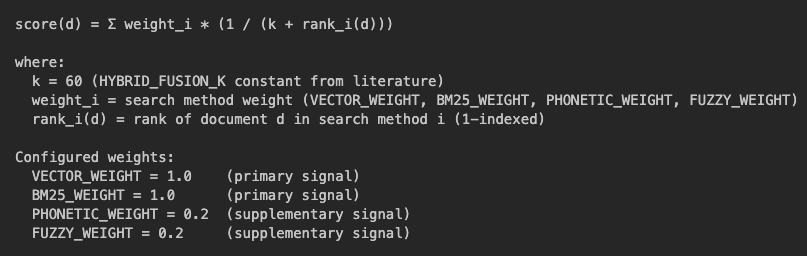
\includegraphics[width=1.0\textwidth]{figures/image35.png}
  \caption{Reciprocal Rank Fusion weights for hybrid retrieval signals}
  \label{fig:fig35}
\end{figure}

The RRF approach provides score normalization across heterogeneous retrieval methods, including semantic, keyword, phonetic, and fuzzy signals, and remains robust to inherent score scale differences between these components. Its weighted formulation further enables explicit prioritization of primary retrieval signals (e.g., semantic and BM25) while still incorporating supplementary signals (e.g., phonetic and fuzzy) to improve recall under ASR noise.\cite{cormack2009reciprocal} In addition, RRF is well-established in information retrieval literature, straightforward to implement, and computationally efficient, making it suitable for low-latency retrieval pipelines. Overall, it effectively combines complementary retrieval strengths to produce a more accurate and ASR-robust candidate set for downstream reranking and generation.

\textbf{4.2.3.3 Stage 3: Cross-Encoder Reranking}

Stage 3 applies a cross-encoder neural reranking model to re-score the candidates retrieved from RRF fusion, providing a final precision-focused refinement step. While the retrieval methods in Stage 1 (vector search, BM25, phonetic, fuzzy) and the fusion algorithm in Stage 2 (RRF) cast a wide net to maximize recall, cross-encoder reranking applies a more computationally expensive but significantly more accurate relevance model to select the final top-k chunks for context assembly.

\textbf{Cross-Encoder vs Bi-Encoder Architecture}

The distinction between bi-encoder and cross-encoder architectures is fundamental to understanding why reranking improves retrieval quality. Bi-encoder models (such as the Jina embedding model used for vector search) independently encode the query and documents into fixed-length vectors, then compute similarity via cosine distance.\cite{jina_embeddings_v3} This approach enables fast retrieval through pre-computed document embeddings and efficient vector search, but it lacks the capacity to model fine-grained query-document interactions because the query and document are encoded separately without mutual attention.

Cross-encoder models, in contrast, jointly encode the query and document as a single concatenated input, allowing the transformer layers to model token-level interactions between query terms and document terms.\cite{nogueira2019passage} This bidirectional attention mechanism enables the model to capture nuanced relevance signals such as term proximity, phrase matching, and semantic entailment that bi-encoders cannot represent. However, cross-encoders require inference for every query-document pair, making them prohibitively expensive for initial retrieval over large corpora. The two-stage retrieval architecture (bi-encoder for fast retrieval $\rightarrow$ cross-encoder for precise reranking) balances efficiency and precision by applying the slow but accurate cross-encoder only to a small candidate set (30-40 chunks from RRF fusion).

\textbf{Reranker Service Configuration and Initialization}

The reranking functionality is implemented as a separate microservice, hosted via llama.cpp server. This separation from the main LLM service and embedding service enables independent scaling and resource allocation for each component.

\textbf{HTTP Request Construction and Payload Preparation}

At reranking time, the system constructs an HTTP POST request containing the query string and the list of candidate document texts. Figure \ref{fig:fig37a} shows the payload preparation logic: the page\_content field is extracted from each LangChain Document object to create a list of plain text strings, which are then packaged into a JSON payload along with the model name and query. The optional top\_n parameter, if provided, is included in the payload to instruct the server to return only the top-n results (though the client enforces this limit locally as well to ensure consistency).

\begin{figure}[H]
  \centering
  
\includegraphics[width=1.0\textwidth]{figure37a.png}
  \caption{Request payload preparation}
  \label{fig:fig37a}
\end{figure}

\textbf{Response Parsing and Score-Based Sorting}

The reranker service returns a JSON response containing a list of results, where each result includes an index (referring to the position in the input documents array) and a relevance\_score (typically in the range [0, 1], with higher scores indicating greater relevance). Figure \ref{fig:fig38a} shows the expected response format.

\begin{figure}[H]
  \centering
  
\includegraphics[width=1.0\textwidth]{figure38a.png}
  \caption{Expected response format}
  \label{fig:fig38a}
\end{figure}

Although the reranker service typically returns results pre-sorted by relevance score, the client explicitly sorts the results to ensure consistency regardless of server implementation, as shown in Figure \ref{fig:fig38b}. The sorted function orders results by the relevance\_score field in descending order (highest scores first), with a fallback to 0 if the score is missing.

\begin{figure}[H]
  \centering
  
\includegraphics[width=1.0\textwidth]{figure38b.png}
  \caption{Sorting by relevance score}
  \label{fig:fig38b}
\end{figure}

\textbf{Metadata Preservation and Document Reconstruction}

After sorting, the system maps the reranked indices back to the original Document objects, preserving all metadata while adding the rerank\_score field, as demonstrated in Figure \ref{fig:fig38c}. For each result, the index is validated to ensure it falls within the bounds of the input documents array, then the corresponding document is retrieved. A new Document object is constructed with the same page\_content and a merged metadata dictionary that includes all original fields (chunk\_id, transcript\_id, timestamps, etc.) plus the new rerank\_score. This metadata preservation ensures that downstream components (context formatting, LLM prompts) can access both the original chunk information and the reranking score.

\begin{figure}[H]
  \centering
  
\includegraphics[width=1.0\textwidth]{figure38c.png}
  \caption{Mapping results to original documents}
  \label{fig:fig38c}
\end{figure}

Finally, the top\_n limit is enforced locally by slicing the reranked\_docs list, as shown in Figure \ref{fig:fig38d}. This client-side enforcement is necessary because not all reranking servers respect the top\_n parameter in the request payload, and it provides a consistent guarantee that exactly top\_n (or fewer, if the input was smaller) documents are returned.

\begin{figure}[H]
  \centering
  
\includegraphics[width=1.0\textwidth]{figure38d.png}
  \caption{Top-n selection}
  \label{fig:fig38d}
\end{figure}

Key advantages of cross-encoder reranking include significantly improved relevance precision compared to bi-encoder similarity or keyword-based scoring, the ability to capture fine-grained semantic entailment and term proximity signals, and robustness to lexical variation (paraphrasing, synonyms) that BM25 cannot handle. The main trade-off is computational cost: cross-encoder inference requires $O(n)$ forward passes for $n$ candidate documents, whereas bi-encoder similarity requires only a single query encoding plus $O(1)$ vector lookups. The two-stage architecture mitigates this cost by limiting cross-encoder reranking to a small candidate set (30-40 chunks from RRF fusion), keeping reranking latency manageable.

\subsection{Context Assembly and Prompt Construction}

After the retrieval and reranking stages produce a ranked list of relevant document chunks, these chunks must be transformed into a structured context string suitable for LLM consumption. Context assembly involves formatting the retrieved chunks with appropriate metadata headers, concatenating them in a readable format, and injecting the result into a prompt template that defines the assistant's behavior and constraints. This section describes the implementation of context formatting, prompt template design, and LLM invocation for answer generation.

\textbf{4.2.4.1 Context Formatting}

The context formatting layer transforms raw Document objects into a structured text representation that the LLM can interpret effectively. Figure \ref{fig:fig40a} demonstrates the formatting implementation, which processes each document individually and constructs a header containing the chunk ID, timestamp range, and sequential position within the result set. Each chunk is formatted as a header line followed by its content, with chunks separated by double newlines for clear visual separation. The header format provides the LLM with temporal context (start and end times) and positional information (chunk ID and position in ranked list), enabling it to reference specific chunks in its responses if needed.

\begin{figure}[H]
  \centering
  
\includegraphics[width=1.0\textwidth]{figure40a.png}
  \caption{Chunk formatting with individual metadata headers}
  \label{fig:fig40a}
\end{figure}

Figure \ref{fig:fig40b} shows an example of the output format for a single document.

\begin{figure}[H]
  \centering
  
\includegraphics[width=1.0\textwidth]{figure40b.png}
  \caption{Output Format Example}
  \label{fig:fig40b}
\end{figure}

The timestamp format follows the SRT standard, preserving millisecond precision from the original transcript. This enables users to locate specific segments in the source audio or video if they wish to verify the LLM's answers. The chunk ID field corresponds to the sequential position of the chunk within its source transcript, allowing for precise cross-referencing with the original document.

\textbf{Citation Formatting for User Transparency}

In addition to formatting context for the LLM, the system provides a citation formatting function that generates structured metadata for user-facing displays, as shown in Figure \ref{fig:fig40d}. This function returns both the formatted context string and a list of source citations, each containing the chunk ID, timestamp, source filename, transcript ID, and a preview of the chunk content. The citation information enables web interfaces to display retrieval provenance alongside generated answers, allowing users to verify the LLM's responses against the source material and explore the full context if needed.

\begin{figure}[H]
  \centering
  
\includegraphics[width=1.0\textwidth]{figure40d.png}
  \caption{Citation formatting for user transparency and source attribution}
  \label{fig:fig40d}
\end{figure}

The preview field contains the first 100 characters of each chunk, providing users with a quick glimpse of the content without requiring them to expand the full text. The full\_text field preserves the complete chunk content for detailed inspection. This dual-level presentation balances information density with accessibility, enabling users to quickly scan sources while retaining the ability to dive deeper when necessary.

\textbf{4.2.4.2 Prompt Templates}

The prompt template layer defines the structure and content of messages sent to the LLM, including the system message that sets the assistant's role and behavior, the human message that contains the user's question, and placeholders for dynamic content such as retrieved context and conversation history. The system uses LangChain's ChatPromptTemplate abstraction to construct multi-turn conversation prompts with type-safe variable substitution.\cite{langchain_prompts,langchain_chatprompt}

\textbf{System Message Design}

Figure \ref{fig:fig42a} shows the RAG system message template, which establishes the assistant's role as a helpful agent with access to transcript excerpts and defines explicit constraints on its behavior. The system message includes three key components: (1) a role definition ("You are a helpful assistant"), (2) a context injection placeholder (\{retrieved\_context\}), and (3) behavioral constraints that ground the LLM's responses in the provided context and prohibit hallucination.

\begin{figure}[H]
  \centering
  
\includegraphics[width=1.0\textwidth]{figure42a.png}
  \caption{RAG system message template defining assistant role and constraints}
  \label{fig:fig42a}
\end{figure}

The grounding instruction ("Use these excerpts to answer the user's questions") explicitly directs the LLM to base its responses on the provided context rather than relying solely on parametric knowledge. The transparency instruction ("If the answer cannot be found in the provided excerpts, say so clearly") encourages the LLM to admit when it lacks sufficient information, reducing the risk of plausible but incorrect answers. The hallucination prevention directive ("Do not make up information not present in the excerpts") reinforces these constraints, explicitly forbidding fabrication. This combination of positive instructions (what to do) and negative constraints (what not to do) has proven effective in reducing hallucination rates in empirical testing.

\textbf{Human Message Template and Reasoning Suppression}

Figure \ref{fig:fig42b} demonstrates the human message template, which contains the user's question followed by the /no\_think directive. This directive is specific to Qwen and similar models that support chain-of-thought reasoning via <think>...</think> tags.\cite{qwen3_thinking_switch} When /no\_think is appended to the input, the model suppresses the output of explicit reasoning steps, producing only the final answer. This improves response cleanliness for end users, who typically do not need to see the model's internal reasoning process.

\begin{figure}[H]
  \centering
  
\includegraphics[width=1.0\textwidth]{figure42b.png}
  \caption{Human message template with reasoning suppression directive}
  \label{fig:fig42b}
\end{figure}

\textbf{Multi-Turn Chat Prompt Construction}

Figure \ref{fig:fig42c} shows how the system message and human message templates are combined with a chat history placeholder to create a complete multi-turn conversation prompt. The ChatPromptTemplate.from\_messages method constructs a prompt with three components: (1) the system message containing the role definition and context, (2) a placeholder for previous conversation turns, and (3) the current human message with the user's question.\cite{langchain_chatprompt,langchain_messages_placeholder}

\begin{figure}[H]
  \centering
  
\includegraphics[width=1.0\textwidth]{figure42c.png}
  \caption{Complete RAG chat prompt construction with history support}
  \label{fig:fig42c}
\end{figure}

The chat history placeholder enables multi-turn interactions where the LLM can reference previous questions and answers when responding to follow-up queries. For example, if the user asks "What is the project timeline?" followed by "Who is responsible for Phase 2?", the LLM can interpret "Phase 2" in the context of the earlier question about the timeline. This capability is essential for natural conversational interactions, as it eliminates the need for users to repeat context with each query.

\textbf{Chat History Structure}

Figure \ref{fig:fig42d} illustrates how chat history is structured using LangChain's message types. Each conversation turn is represented as a HumanMessage (user input) or AIMessage (assistant response), and these messages are accumulated in a list that is injected into the chat\_history placeholder.\cite{langchain_messages_placeholder} The LLM receives the entire conversation history along with the current question, enabling it to maintain context across multiple turns. This approach supports pronouns, follow-up questions, and clarifications that reference earlier parts of the conversation.

\begin{figure}[H]
  \centering
  
\includegraphics[width=1.0\textwidth]{figure42d.png}
  \caption{Chat history structure for multi-turn conversation support}
  \label{fig:fig42d}
\end{figure}

The chat history is reset when the user starts a new conversation or switches to a different transcript, ensuring that context from unrelated queries does not leak into subsequent interactions. The system limits history length to the most recent N turns (e.g., last 5 exchanges) to prevent the prompt from exceeding the LLM's context window, though this constraint is rarely reached in practice given the short length of typical question-answer pairs.

\textbf{Streaming Response Handling}

Figure \ref{fig:fig43d} demonstrates streaming invocation using the chain.stream method. Instead of returning a single string containing the complete response, the stream method returns a generator that yields tokens incrementally as they are produced by the LLM. This enables real-time display in chat interfaces, where each token is printed immediately upon arrival.

\begin{figure}[H]
  \centering
  
\includegraphics[width=1.0\textwidth]{figure43d.png}
  \caption{Streaming response handling for real-time token display}
  \label{fig:fig43d}
\end{figure}

Streaming mode does not reduce total generation time. The LLM still takes the same amount of time to produce the full response, but it significantly improves perceived responsiveness from the user's perspective. Users see the first tokens quickly, providing immediate feedback that the system is working.

\section{Stretch Goals and Deployment}
This section will be completed in the final report, once everything has been finalized.
